\documentclass{standalone}
\usepackage{tikz}
\usepackage{ctex,siunitx}
\setCJKmainfont{Noto Serif CJK SC}
\usepackage{tkz-euclide}
\usepackage{amsmath}
\usetikzlibrary{patterns, calc,3d}
\usetikzlibrary {decorations.pathmorphing,decorations.pathreplacing,decorations.shapes,}
\tikzset{label style/.append style={font=\small}}
\begin{document}
\small
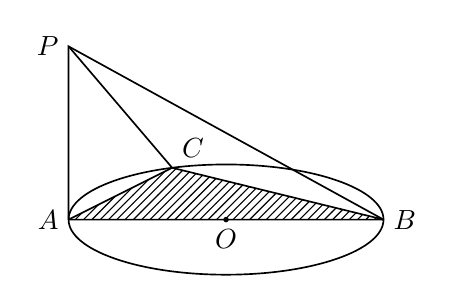
\begin{tikzpicture}[>=latex,scale=1.0]
  \draw[semithick](0,0)ellipse(2 and 0.7)(-2,0)--(2,0)(-2,2.2)--({2*cos(110)},{0.7*sin(110)})node[above right]{$C$};
  \draw[semithick](-2,0)node[left]{$A$}--(-2,2.2)node[left]{$P$}--(2,0)node[right]{$B$};
  \draw[semithick,pattern=north east lines](-2,0)--({2*cos(110)},{0.7*sin(110)})--(2,0);
  \fill(0,0)circle(1pt)node[below]{$O$};
\end{tikzpicture}
\end{document}